\chapter{Entwurfsmuster}
    WPSflow behilft sich sowohl serverseitig, als auch clientseitig mit diversen Frameworks - hauptsächlich Django für den HTTP Server und Angular für die Web-App. Daher müssen wenige Enwurfsmuster selber geschrieben werden, sondern die vorhandenen Schnittstellen der Frameworks genutzt werden. Dennoch haben sich ein Paar nützliche Entwurfsmuster aus dem Klassendiagramm herauskristallisiert.

    \section{Strategy}
    Das Format der Artefakte hängt von den Resultaten eines WPS Prozesses ab. Diese Resultate können verschiedene Formen annehmen, wobei wir die Häufigsten abdecken wollen - diese sind XML, JSON und Bilder. 
    Dieses Problem wird mit dem Strategy-Entwurfmuster (Abbildung \ref{fig:pattern_strategy_diagramm}) gelöst.
    Falls ein Task fehlschlägt, wird dieser durch die Klasse ErrorRepresentation dem Benutzer angezeigt. Nicht behandelte Formate werden je nach Dateigröße als Raw-String angezeigt oder zum Download angeboten.
    
    \begin{figure}[h]
        \centering
        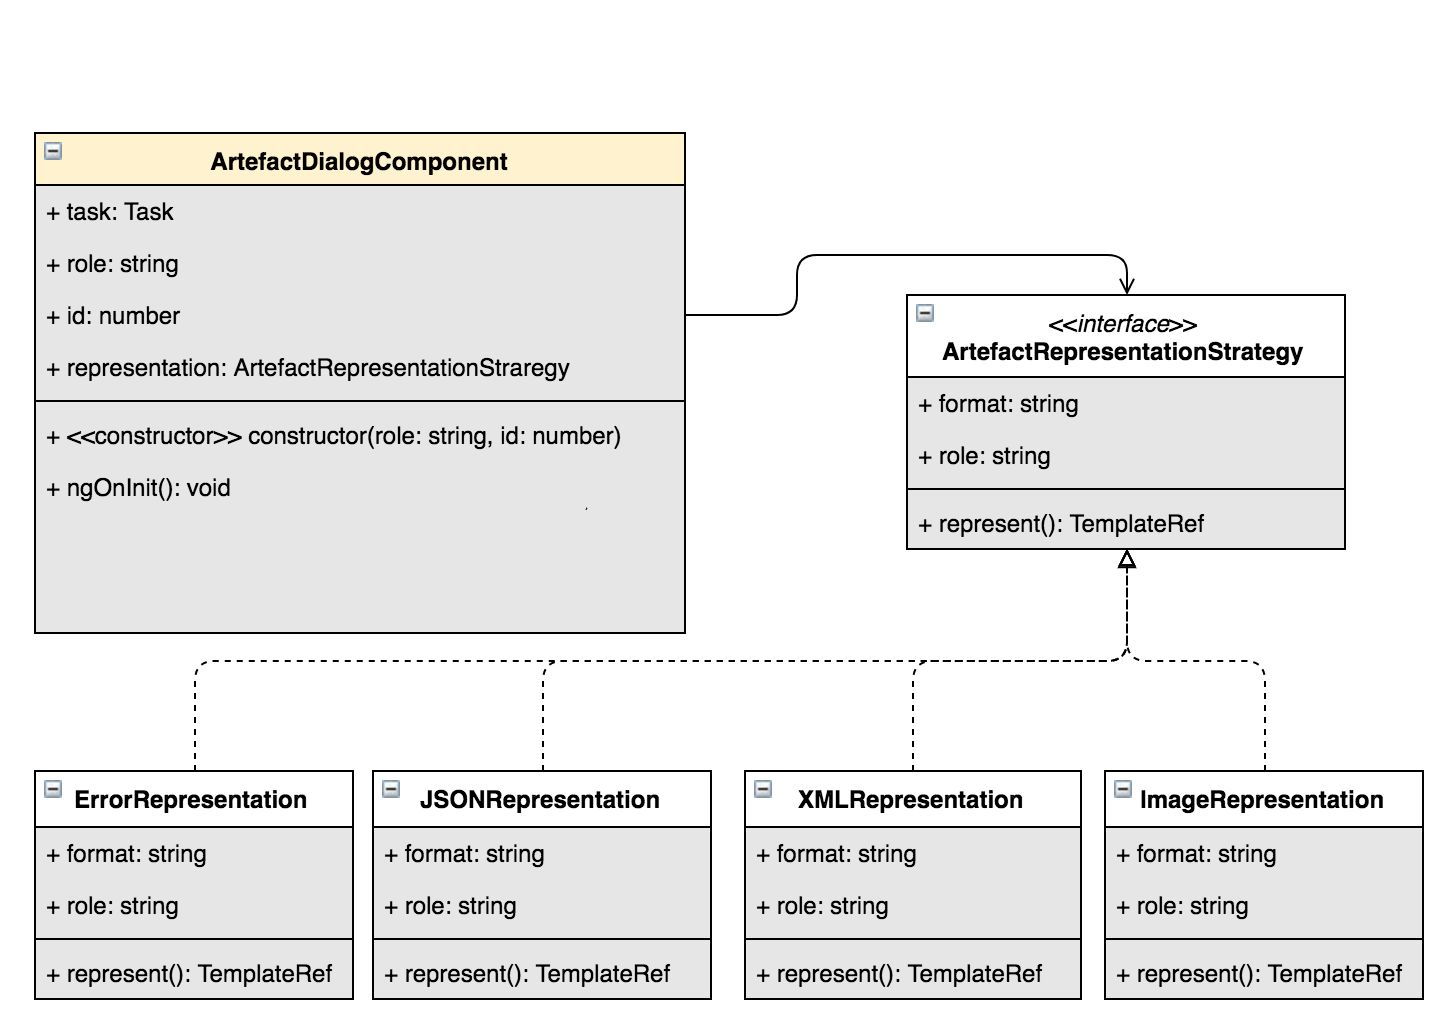
\includegraphics[width=15cm]{diagrams/pattern_strategy.png}
        \caption{Verwendung der Strategy-Entwurfmusters im Frontend}
        \label{fig:pattern_strategy_diagramm}
    \end{figure}
    
    \section{Object Pool}
    Es werden keine HTTP Request von Client-Komponenten geschickt, hierfür sind stattdessen Services (Abbildung \ref{fig:pattern_pool_diagramm}) zuständig. Sie bieten den Komponenten eine Schnittstelle zum Erstellen, Bearbeiten und Löschen von Daten.
    
     \begin{figure}[h]
        \centering
        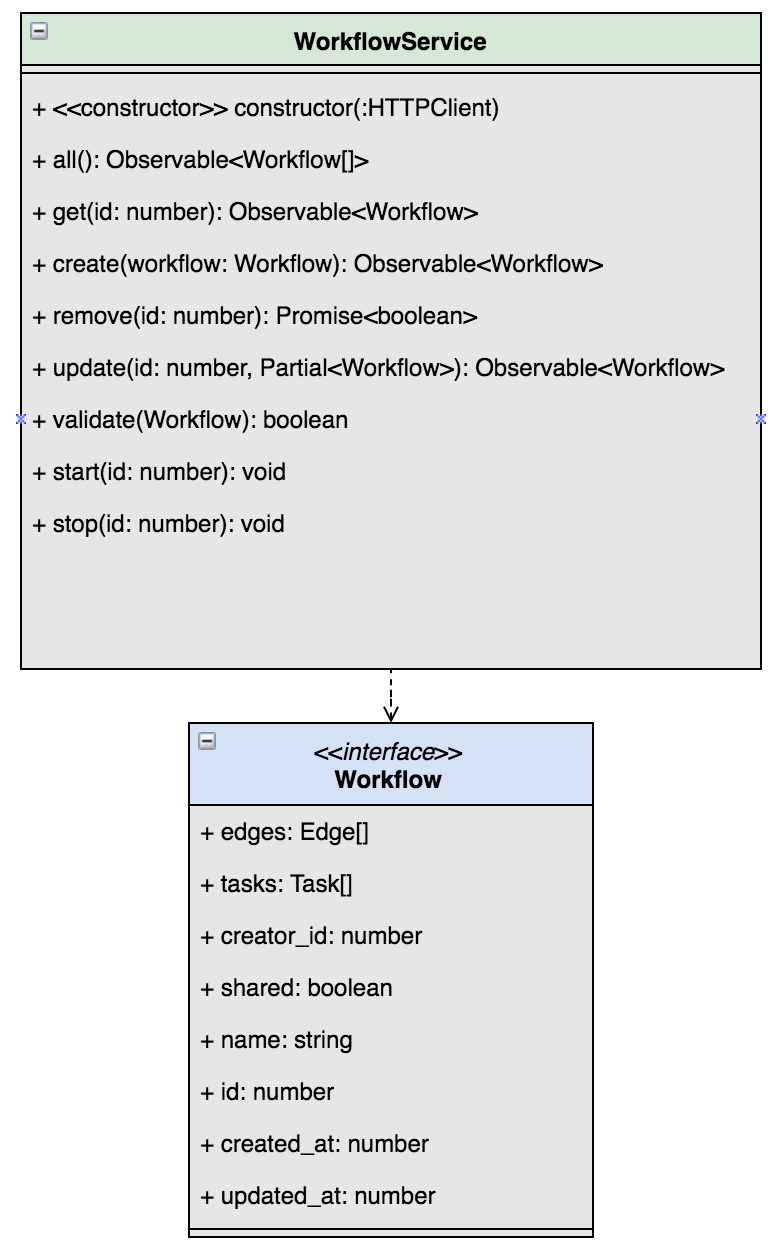
\includegraphics[width=8cm]{diagrams/pattern_pool.png}
        \caption{Beispiel eines Object Pools (hier für Workflows)}
        \label{fig:pattern_pool_diagramm}
    \end{figure}
    
    \section{Observer}
    Der Client hält seine Daten aktuell, indem er in regelmäßigen Abständen Anfragen an den Django Server schickt. Um die Aktualisierung der Daten möglichst angenehm zu halten, werden Observables benutzt. Wir benutzen hierfür eine schon fertige Implementierung von rxjs.
    Beispiel siehe WorkflowService in Abbildung \ref{fig:pattern_pool_diagramm}
	